% Compile from this directory: latexmk -pdf -interaction=nonstopmode -halt-on-error main.tex
\documentclass[11pt]{article}
\usepackage[T1]{fontenc}
\usepackage[utf8]{inputenc}
\usepackage[english]{babel}
\usepackage{lmodern}
\usepackage[a4paper,margin=2.1cm]{geometry}
\usepackage{microtype}
\usepackage{amsmath,amssymb,mathtools}
\usepackage{booktabs,array,tabularx}
\usepackage{enumitem}
\usepackage{xcolor}
\usepackage{hyperref}
\usepackage[most]{tcolorbox}
\usepackage{tikz}
\usetikzlibrary{arrows.meta,positioning,calc}
\usepackage{listings}
\usepackage{fancyhdr}
\usepackage{lastpage}
\usepackage{siunitx}
\sisetup{detect-all}

\definecolor{navy}{HTML}{17365D}
\definecolor{pale}{HTML}{EFF4FA}
\definecolor{forest}{HTML}{246448}
\definecolor{mint}{HTML}{EDF7F1}
\definecolor{amber}{HTML}{80510E}
\definecolor{cream}{HTML}{FFF8E9}
\hypersetup{colorlinks=true,linkcolor=navy,urlcolor=navy,pdftitle={LDS1071 - Fully Solved Midterm II Study Guide},pdfauthor={Study material}}
\setlength{\parindent}{0pt}
\setlength{\parskip}{5pt}
\setlength{\headheight}{14pt}
\setlist[enumerate]{leftmargin=2.0em,itemsep=3pt,topsep=3pt}
\setlist[itemize]{leftmargin=1.6em,itemsep=2pt,topsep=3pt}
\pagestyle{fancy}
\fancyhf{}
\lhead{LDS1071 --- Midterm II}
\rhead{Worked study guide}
\cfoot{\thepage\ / \pageref{LastPage}}

\newtcolorbox{answer}{breakable,colback=mint,colframe=forest,boxrule=.65pt,arc=1.2mm,left=2mm,right=2mm,top=1mm,bottom=1mm}
\newtcolorbox{important}{breakable,colback=cream,colframe=amber,boxrule=.6pt,arc=1mm,left=2mm,right=2mm,top=1mm,bottom=1mm,title=Important distinction,fonttitle=\bfseries}
\newtcolorbox{problem}{breakable,colback=white,colframe=navy,boxrule=.75pt,arc=1.2mm,left=2.8mm,right=2.8mm,top=1.5mm,bottom=1.5mm,title=Problem --- faithful English translation of the practice guide,fonttitle=\bfseries}
\newtcolorbox{worked}{breakable,colback=pale,colframe=navy,boxrule=.75pt,arc=1.2mm,left=2.8mm,right=2.8mm,top=1.5mm,bottom=1.5mm,title=Additional worked example (from lecture material),fonttitle=\bfseries}
\newtcolorbox{concept}{breakable,colback=pale,colframe=navy,boxrule=.6pt,arc=1mm,left=2mm,right=2mm,top=1mm,bottom=1mm,title=Underlying idea,fonttitle=\bfseries}
\newcommand{\subq}[1]{\subsection*{#1}}
\newcommand{\E}{\mathbb E}
\newcommand{\Var}{\operatorname{Var}}
\newcommand{\Cov}{\operatorname{Cov}}
\newcommand{\R}{\mathbb R}
\newcommand{\given}{\,\middle|\,}
\newcommand{\norm}[1]{\left\lVert#1\right\rVert}
\newcommand{\abs}[1]{\left\lvert#1\right\rvert}
\newcommand{\argmin}{\operatorname*{arg\,min}}
\newcommand{\argmax}{\operatorname*{arg\,max}}
\newcommand{\dd}{\mathrm d}
\lstset{language=Python,basicstyle=\ttfamily\footnotesize,backgroundcolor=\color{black!3},frame=single,rulecolor=\color{black!15},keywordstyle=\color{navy}\bfseries,commentstyle=\color{forest},showstringspaces=false,columns=fullflexible,breaklines=true,keepspaces=true}

\title{\textbf{Midterm II --- Fully Solved Study Guide}\\[2mm]\large Machine Learning (LDS1071)}
\author{Step-by-step calculations, explanations, and formula reference}
\date{}

\begin{document}
\maketitle
\begin{concept}
\textbf{Source and scope.} This document follows the 16 exercises and all their subquestions in the supplied five-page \emph{Gu\'ia de Estudio --- Examen parcial II} for LDS1071. Numerical givens are preserved. Answers are presented in English for studying, while original Spanish document tokens (e.g., \texttt{modelo}, \texttt{red}) are retained. The source guide describes these as \emph{practice} questions, not an exhaustive examination syllabus.
\end{concept}
\tableofcontents
\clearpage

\section*{Notation and essential vocabulary}
\addcontentsline{toc}{section}{Notation and essential vocabulary}
Let $n$ denote the number of observations, $p$ the number of features, and $K$ the number of clusters. The dataset is $X=\{x_i\}_{i=1}^{n}$, with $x_i\in\R^p$; $c(i)$ denotes the cluster assigned to observation $i$; and $\mu_k$ denotes centroid $k$. We write $\norm{v}_2$ for Euclidean norm, $\norm{v}_2^2$ for its square, $\lambda_j$ for an eigenvalue, and $\hat y_i$ for a predicted label.

\textbf{Glossary.} A \emph{centroid} is a cluster's arithmetic mean; \emph{inertia} is within-cluster sum of squared distances; \emph{linkage} specifies distance between clusters; a \emph{manifold} is a locally low-dimensional surface that may curve inside a higher-dimensional space; a \emph{mixture responsibility} is a component's conditional probability for an observation; \emph{data leakage} is information from validation or test data improperly used during model fitting; a \emph{BPE merge} combines the most frequent adjacent token pair within word boundaries; \emph{IDF} weights terms by document rarity; a \emph{paired resample} preserves alignment of outcomes and both models' predictions for each observation.

\begin{important}
\textbf{How to study.} For each exercise, reproduce the calculation without looking at the answer, then explain \emph{why} its formula is appropriate. The complete formula reference appears in Appendix~\ref{sec:formulas}.
\end{important}
\clearpage

% Each exercise begins on its own new page, even when the preceding exercise ends mid-page.
% One exercise per included source file; numbering follows the supplied guide.
\clearpage
\section{One iteration of $K$-means}
\label{sec:ex1}
\begin{problem}
One-dimensional observations are $X=\{1,3,9,12\}$, with $K=2$ and initial centroids $\mu_1^{(0)}=1$, $\mu_2^{(0)}=12$.
\begin{enumerate}[label=\textbf{(\alph*)}]
\item Assign each observation to its nearest centroid using Euclidean distance.
\item Compute the updated centroids $\mu_1^{(1)}$ and $\mu_2^{(1)}$.
\item Calculate inertia $\sum_i\norm{x_i-\mu_{c(i)}}_2^2$ using the \emph{updated} centroids.
\item If you repeat assignment with those updated centroids, does any cluster membership change? Explain.
\end{enumerate}
\end{problem}


\begin{concept}
$K$-means alternates two operations: (i) assign each point to its nearest centroid; (ii) replace each centroid with its assigned points' arithmetic mean. Its objective is the \emph{within-cluster sum of squares} $J=\sum_i\norm{x_i-\mu_{c(i)}}_2^2$.
\end{concept}

\subq{(a) Assign each point to its closest initial centroid}
In one dimension, Euclidean distance is absolute difference: $d(x,\mu)=\abs{x-\mu}$. Compute both distances before choosing the smaller value:
\begin{center}
\begin{tabular}{@{}rrrrl@{}}\toprule
$x_i$ & $\abs{x_i-1}$ & $\abs{x_i-12}$ & Nearest & Assignment\\\midrule
1&0&11&1&$C_1$\\
3&2&9&1&$C_1$\\
9&8&3&2&$C_2$\\
12&11&0&2&$C_2$\\\bottomrule
\end{tabular}
\end{center}
Thus $C_1=\{1,3\}$ and $C_2=\{9,12\}$.

\subq{(b) Update the centroids}
Take the mean of each assigned cluster:
\[
\mu_1^{(1)}=\frac{1+3}{2}=\boxed{2},\qquad
\mu_2^{(1)}=\frac{9+12}{2}=\boxed{10.5}.
\]
The updated centroids minimize the within-cluster squared-error objective \emph{for the current assignments}.

\subq{(c) Calculate the inertia using the \emph{updated} centroids}
Substitute each point's assigned, updated centroid into the specified objective:
\begin{align*}
J^{(1)}&=(1-2)^2+(3-2)^2+(9-10.5)^2+(12-10.5)^2\\
&=1+1+2.25+2.25=\boxed{6.5}.
\end{align*}
Note that this is a \emph{sum}, not a mean; do not divide by four.

\subq{(d) Reassign using the updated centroids}
The nearest-centroid decision boundary in one dimension is their midpoint:
\[
b=\frac{2+10.5}{2}=6.25.
\]
Values $1$ and $3$ are less than $6.25$; $9$ and $12$ exceed it. Consequently the assignments remain $\{1,3\}$ and $\{9,12\}$. A subsequent centroid update also gives $2$ and $10.5$: this solution has reached a fixed point of the alternating algorithm.
\begin{answer}
\textbf{Result:} $C_1=\{1,3\}$, $C_2=\{9,12\}$; centroids $(2,10.5)$; inertia $6.5$; no further assignment changes.
\end{answer}

\clearpage
\section{Selecting the number of clusters with the elbow method}
\label{sec:ex2}
\textbf{Given:}
\begin{center}\begin{tabular}{@{}rrrrrr@{}}\toprule $K$&1&2&3&4&5\\\midrule Inertia&900&440&210&185&170\\\bottomrule\end{tabular}\end{center}

\subq{(a) Which $K$ does the elbow method suggest?}
The elbow heuristic favors the point beyond which the decrease in inertia becomes much smaller. Calculate successive improvements:
\[
\begin{aligned}
\Delta J_{1\to2}&=900-440=460,\\
\Delta J_{2\to3}&=440-210=230,\\
\Delta J_{3\to4}&=210-185=25,\\
\Delta J_{4\to5}&=185-170=15.
\end{aligned}
\]
After $K=3$, each extra cluster gives only modest improvement compared with previous increments. Hence $\boxed{K=3}$ is the natural elbow choice for these values. This is a qualitative heuristic, not a statistical proof or a uniquely defined optimization rule.

\subq{(b) Why not always choose the smallest inertia?}
Adding centroids cannot increase the \emph{globally minimized} $K$-means objective; with one centroid per data point, inertia can reach zero. Thus minimizing training inertia across all $K$ systematically favors unnecessarily large $K$. We care about a parsimonious and interpretable partition, not just low training distortion. In practical runs, different local optima can cause small numerical irregularities, so repeated initialization is useful.

\subq{(c) Another evaluation and one limitation}
The \emph{average silhouette coefficient} compares a point's mean within-cluster distance $a(i)$ with its mean distance $b(i)$ to the closest other cluster:
\[
s(i)=\frac{b(i)-a(i)}{\max\{a(i),b(i)\}}\in[-1,1].
\]
Higher values often indicate greater geometric separation. \textbf{Limitation:} silhouette evaluates a distance geometry, not whether categories are scientifically meaningful; it can also disadvantage elongated, nested, or irregularly shaped clusters. For large datasets, pairwise distance computation may be expensive.

\begin{answer}
The elbow suggests $\boxed{K=3}$. Validate it using silhouette, partition stability, cluster sizes, and domain interpretation rather than inertia alone.
\end{answer}

\clearpage
\section{DBSCAN and noise observations}
\label{sec:ex3}
\textbf{Given:} Two dense, curved bands in two dimensions, some isolated points, and approximately comparable local densities within the bands.

\subq{(a) Why might DBSCAN be preferable to $K$-means?}
$K$-means assigns every point to a nearest centroid. Its Euclidean-distance, centroid-based partitions are Voronoi regions, so a curved band may be split unnaturally; distant outliers also receive cluster assignments. In contrast, DBSCAN groups points connected through sufficiently dense neighborhoods, which can follow curved or non-convex shapes. DBSCAN also explicitly detects sparse observations as noise, without requiring a predetermined $K$.

\subq{(b) Define a core point and the roles of $\varepsilon$ and \texttt{min\_samples}}
For a candidate point $x_i$, define its closed $\varepsilon$-neighborhood:
\[
N_{\varepsilon}(x_i)=\{x_j:\norm{x_j-x_i}_2\leq\varepsilon\}.
\]
A point is \emph{core} when $\abs{N_{\varepsilon}(x_i)}\geq m$, where $m=\texttt{min\_samples}$. \textbf{The point itself counts} as one of the $m$ neighbors, as specified in the question. Core points connected through chains of neighboring core points form the dense skeleton of a cluster. Non-core points sufficiently close to a core point may be \emph{border points}; points that cannot be reached from a core point are labeled \emph{noise}.

\subq{(c) What happens if $\varepsilon$ becomes very large?}
For fixed $m$, larger $\varepsilon$ means larger neighborhoods. More observations become core or border points; isolated points may cease to be noise; and formerly distinct dense regions may merge through density-connected paths. If $\varepsilon$ is sufficiently large compared with all pairwise distances and there are at least $m$ total observations, all points can be assigned to one cluster. Therefore a large $\varepsilon$ can destroy the desired two-band distinction.

\subq{(d) Meaning of Scikit-Learn label $-1$}
In \texttt{DBSCAN.labels\_}, $-1$ identifies an observation classified as noise under the selected metric, $\varepsilon$, and \texttt{min\_samples}. It is not a numbered cluster, nor does it prove the observation is objectively anomalous independent of these choices.
\begin{answer}
DBSCAN is useful for comparable-density, non-convex clusters and noise. It is sensitive to neighborhood scale and may struggle when clusters have strongly different densities.
\end{answer}

\clearpage
\section{Gaussian mixture models: interpretation, BIC, and AIC}
\label{sec:ex4}
\textbf{Given:} Partially overlapping elliptical groups; model-selection scores:
\begin{center}\begin{tabular}{@{}rrrrr@{}}\toprule Components&1&2&3&4\\\midrule BIC&790&620&574&590\\ AIC&775&585&520&515\\\bottomrule\end{tabular}\end{center}

\subq{(a) Which component count is selected by each criterion?}
Both criteria are minimized, not maximized. For BIC, the minimum is $\boxed{574}$ at $\boxed{K=3}$. For AIC, the minimum is $\boxed{515}$ at $\boxed{K=4}$. Different choices are possible because they penalize complexity differently; no sample size or parameter counts are supplied here for decomposing their numerical values.

\subq{(b) Why can a GMM represent these data better than $K$-means?}
A Gaussian mixture specifies a distribution rather than only a nearest-centroid partition:
\[
p(x)=\sum_{k=1}^{K}\pi_k\,\mathcal N(x\mid\mu_k,\Sigma_k),\qquad
\pi_k\geq0,\quad \sum_k\pi_k=1.
\]
Each covariance matrix $\Sigma_k$ can represent an elliptical orientation and spread. Overlapping components may assign positive probability to the same observation, unlike $K$-means' hard membership. This flexibility can be advantageous for elliptical overlapping groups, though the Gaussian-family assumption may be wrong for other shapes.

\subq{(c) Meaning of a component-membership probability of $0.7$}
The posterior \emph{responsibility} for component $k$ is
\[
\gamma_{ik}=P(Z_i=k\mid x_i)
=\frac{\pi_k\mathcal N(x_i\mid\mu_k,\Sigma_k)}{\sum_{\ell=1}^{K}\pi_\ell\mathcal N(x_i\mid\mu_\ell,\Sigma_\ell)}.
\]
A value $\gamma_{ik}=0.7$ means that, \emph{conditional on the fitted GMM and the observation}, component $k$ has estimated probability $70\%$ of being the latent generator of $x_i$. The remaining component probabilities sum to $0.3$. It is \emph{not} a statement that the observation is classified correctly with $70\%$ probability.

\subq{(d) BIC's fit--complexity trade-off}
For maximized log-likelihood $\hat\ell$, parameter count $q$, and sample size $n$:
\[
\mathrm{BIC}=q\log n-2\hat\ell,\qquad
\mathrm{AIC}=2q-2\hat\ell.
\]
A more complex model often raises $\hat\ell$ (better training fit) but also increases $q$ (larger penalty). BIC imposes a penalty $\log n$ per parameter, rather than AIC's constant $2$. When $n>e^2\approx7.39$, BIC's per-parameter penalty is larger; neither score is a guarantee that the chosen model is the true data-generating model.
\begin{answer}
Choose $\boxed{3}$ components under BIC and $\boxed{4}$ under AIC. The disagreement illustrates the competing penalties for model complexity.
\end{answer}

\clearpage
\section{Agglomerative clustering: single and complete linkage}
\label{sec:ex5}
\textbf{Given:} $A=0$, $B=3$, $C=7$, $D=13$ on the real line.

\subq{(a) Construct the Euclidean distance matrix}
In one dimension, $d(P,Q)=\abs{P-Q}$. For example, $d(B,D)=\abs{3-13}=10$ and $d(C,D)=\abs{7-13}=6$. Compute every pair and use symmetry:
\[
D=\begin{array}{c|rrrr}
& A & B & C & D\\\hline
A&0&3&7&13\\
B&3&0&4&10\\
C&7&4&0&6\\
D&13&10&6&0
\end{array}.
\]

\subq{(b) Perform the three single-linkage merges}
Single linkage defines intercluster distance by the \emph{nearest cross-cluster pair}:
\[
d_{\mathrm{single}}(U,V)=\min_{u\in U,\,v\in V} d(u,v).
\]
\begin{enumerate}[label=\textbf{Step \arabic*.}]
\item The smallest initial distance is $d(A,B)=3$. Merge $A$ and $B$ to form $\{A,B\}$ at height $3$.
\item Recompute the distances from the new cluster:
\[
\begin{aligned}
d(\{A,B\},C)&=\min\{7,4\}=4,\\
d(C,D)&=6,\\
d(\{A,B\},D)&=\min\{13,10\}=10.
\end{aligned}
\]
The minimum is $4$, so merge $\{A,B\}$ with $C$.
\item The final distance is $d(\{A,B,C\},D)=\min\{13,10,6\}=6$. Merge with $D$ at height $6$.
\end{enumerate}
\begin{center}\begin{tabular}{@{}cll@{}}\toprule Merge&Clusters joined&Height\\\midrule 1&$A$ and $B$&3\\2&$\{A,B\}$ and $C$&4\\3&$\{A,B,C\}$ and $D$&6\\\bottomrule\end{tabular}\end{center}

\subq{(c) Perform the three complete-linkage merges}
Complete linkage uses the \emph{farthest cross-cluster pair}:
\[
d_{\mathrm{complete}}(U,V)=\max_{u\in U,\,v\in V} d(u,v).
\]
\begin{enumerate}[label=\textbf{Step \arabic*.}]
\item Merge $A$ and $B$ at the initial minimum distance $3$.
\item Recalculate $d(\{A,B\},C)=\max\{7,4\}=7$, $d(\{A,B\},D)=\max\{13,10\}=13$, while $d(C,D)=6$. The smallest is now $6$, so merge $C$ and $D$.
\item The two clusters $\{A,B\}$ and $\{C,D\}$ have distance $\max\{7,13,4,10\}=13$. Merge at height $13$.
\end{enumerate}
\begin{center}\begin{tabular}{@{}cll@{}}\toprule Merge&Clusters joined&Height\\\midrule 1&$A$ and $B$&3\\2&$C$ and $D$&6\\3&$\{A,B\}$ and $\{C,D\}$&13\\\bottomrule\end{tabular}\end{center}
The source specifies alphabetical tie-breaking. No equal minimum distances arise during these particular merges, so the tie rule is not needed.

\subq{(d) Compare the results and explain each distance}
\textbf{Single linkage} can join clusters through a short chain of close observations (the \emph{chaining effect}); its final height is $6$. \textbf{Complete linkage} requires controlling the largest separation between members, often favoring tighter groups; its final height is $13$. Different linkage functions encode different notions of what makes two clusters close.
\begin{answer}
\textbf{Single:} $AB$ at $3$; $(AB)C$ at $4$; $(ABC)D$ at $6$.\\
\textbf{Complete:} $AB$ at $3$; $CD$ at $6$; $(AB)(CD)$ at $13$.
\end{answer}

\clearpage
\section{Reading and drawing a dendrogram}
\label{sec:ex6}
\textbf{Given merges:} $A$ with $B$ at height $1$; $D$ with $E$ at $2$; $\{A,B\}$ with $C$ at $4$; and $\{A,B,C\}$ with $\{D,E\}$ at $9$.

\subq{(a) Draw a dendrogram with the specified heights}
The vertical coordinate records the linkage height at which two clusters join. The branches below reproduce the exact merge sequence:
\begin{center}
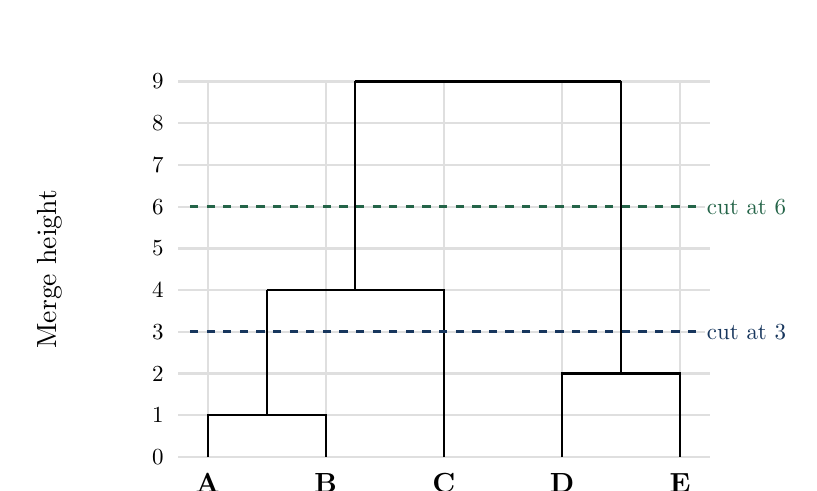
\begin{tikzpicture}[x=1.5cm,y=.53cm,line width=.8pt]
  \draw[gray!25] (-.25,0) grid[xstep=1,ystep=1] (4.25,9);
  \foreach \y in {0,1,2,3,4,5,6,7,8,9} {\node[left,scale=.83] at (-.3,\y) {\y};}
  \node[rotate=90,anchor=south] at (-1.15,4.5) {Merge height};
  % A,B joined at 1; their representative is at x=.5.
  \draw (0,0)--(0,1)--(1,1)--(1,0);
  \draw (.5,1)--(.5,4);
  % {A,B} joined with C at 4; new representative at x=1.25.
  \draw (2,0)--(2,4)--(.5,4);
  \draw (1.25,4)--(1.25,9);
  % D,E joined at 2; their representative is x=3.5.
  \draw (3,0)--(3,2)--(4,2)--(4,0);
  \draw (3.5,2)--(3.5,9);
  % Final join at 9.
  \draw (1.25,9)--(3.5,9);
  \draw[navy,dashed,line width=1pt] (-.15,3)--(4.15,3);
  \draw[forest,dashed,line width=1pt] (-.15,6)--(4.15,6);
  \foreach \x/\n in {0/A,1/B,2/C,3/D,4/E}{\node[below,font=\bfseries] at (\x,-.15) {\n};}
  \node[navy,right,fill=white,inner sep=1pt,scale=.83] at (4.2,3) {cut at 3};
  \node[forest,right,fill=white,inner sep=1pt,scale=.83] at (4.2,6) {cut at 6};
\end{tikzpicture}
\end{center}
The horizontal positions are schematic; the \emph{heights} and membership relations are the meaningful quantities.

\subq{(b) Cut at height $h=3$}
Merges at heights $1$ and $2$ have already happened. The merge at height $4$ has not. Therefore the three clusters are
\[
\boxed{\{A,B\},\quad \{C\},\quad \{D,E\}}\quad (3\text{ clusters}).
\]

\subq{(c) Cut at height $h=6$}
The height-$4$ merge has also happened, but the height-$9$ merge has not. The clusters are
\[
\boxed{\{A,B,C\},\quad \{D,E\}}\quad (2\text{ clusters}).
\]

\subq{(d) What do merge heights tell us?}
A merge height is the computed \emph{linkage distance} between the two clusters at the moment they join, under the chosen distance metric and linkage method. Large vertical gaps can indicate a comparatively pronounced separation (for this example, $9-4=5$ before the final join). Heights are not probabilities and need not represent a particular member-to-member distance unless the linkage definition makes them so.
\begin{answer}
At height $3$: three clusters $AB$, $C$, $DE$. At height $6$: two clusters $ABC$, $DE$.
\end{answer}

\clearpage
\section{Silhouette coefficient}
\label{sec:ex7}
\begin{problem}
For two observations, the average within-cluster distance $a(i)$ and nearest other-cluster average distance $b(i)$ are:
\begin{center}\begin{tabular}{@{}lrr@{}}\toprule Observation&$a(i)$&$b(i)$\\\midrule $x_1$&3&9\\$x_2$&5&4\\\bottomrule\end{tabular}\end{center}
Use $s(i)=[b(i)-a(i)]/\max\{a(i),b(i)\}$.
\begin{enumerate}[label=\textbf{(\alph*)}]
\item Calculate both silhouette coefficients.
\item Interpret the sign of each coefficient.
\item Does a high average silhouette guarantee meaningful domain-specific groups? Explain.
\end{enumerate}
\end{problem}


\subq{(a) Calculate both silhouettes}
Use the exact formula supplied by the guide:
\[
s(i)=\frac{b(i)-a(i)}{\max\{a(i),b(i)\}}.
\]
For $x_1$, $b=9>a=3$, so the denominator is $9$:
\[
s(x_1)=\frac{9-3}{\max\{3,9\}}=\frac{6}{9}
=\boxed{\frac{2}{3}\approx0.667}.
\]
For $x_2$, $b=4<a=5$, so the denominator is $5$:
\[
s(x_2)=\frac{4-5}{\max\{5,4\}}=-\frac15
=\boxed{-0.2}.
\]

\subq{(b) Interpret the signs}
$x_1$ has a positive silhouette, suggesting that on average it is substantially closer to its own cluster than to its closest competing cluster. $x_2$ has a negative silhouette: on average it lies closer to an alternative cluster than to its assigned one, potentially indicating questionable placement or overlapping groups. A coefficient near $0$ indicates a borderline observation; the range is $[-1,1]$.

\subq{(c) Does a high mean silhouette guarantee domain meaning?}
No. Silhouette quantifies within- versus between-cluster \emph{distance} relationships; it does not test semantic validity, causal explanation, external labels, clinical usefulness, or interpretability. For example, document clusters might separate by document length or writing style while failing to correspond to desired research topics. Domain review, cluster exemplars, stability, and external validation (if available) remain important.
\begin{answer}
$\boxed{s(x_1)\approx0.667}$ indicates good separation; $\boxed{s(x_2)=-0.2}$ suggests possible misassignment or overlap.
\end{answer}


\subsection*{Supplementary worked example: calculate $a(i)$ and $b(i)$ from raw observations}
\begin{reviewproblem}
Consider three \emph{given} clusters on the real number line, with ordinary Euclidean distance
$d(x,y)=|x-y|$:
\[
C_1=\{0,2,7\},\qquad C_2=\{8,9\},\qquad C_3=\{15,18\}.
\]
\begin{enumerate}[label=\textbf{(\alph*)}]
\item Calculate the within-cluster mean distance $a(i)$ and the nearest other-cluster mean distance $b(i)$ for $x_i=2$.
\item Repeat for $x_i=7$ and calculate the silhouette of each observation.
\item Explain why $b(i)$ is \emph{not} simply the distance to the nearest observation in another cluster.
\end{enumerate}
These numbers are a constructed practice example; they are \emph{not} additional observations supplied by the original study guide.
\end{reviewproblem}

\begin{center}
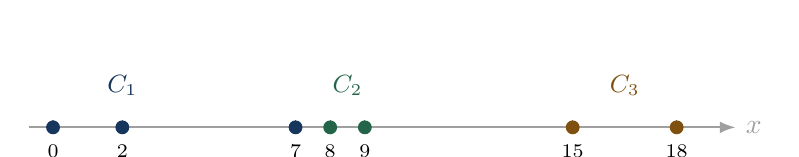
\begin{tikzpicture}[x=0.44cm,y=1cm]
  \draw[-{Latex[length=2mm]},gray!75,thick] (-0.7,0)--(19.7,0) node[right] {$x$};
  \foreach \x in {0,2,7,8,9,15,18}{\draw[gray] (\x,.09)--(\x,-.09);}
  \foreach \x in {0,2,7}{\fill[navy] (\x,0) circle (2.5pt);}
  \foreach \x in {8,9}{\fill[forest] (\x,0) circle (2.5pt);}
  \foreach \x in {15,18}{\fill[amber] (\x,0) circle (2.5pt);}
  \foreach \x in {0,2,7,8,9,15,18}{\node[below=3pt,font=\scriptsize] at (\x,0) {$\x$};}
  \node[above=8pt,text=navy,font=\small] at (2,0) {$C_1$};
  \node[above=8pt,text=forest,font=\small] at (8.5,0) {$C_2$};
  \node[above=8pt,text=amber,font=\small] at (16.5,0) {$C_3$};
\end{tikzpicture}
\end{center}

\textbf{Definitions.} If $C(i)$ is the assigned cluster containing $x_i$, then
\[
\begin{aligned}
a(i)&=\frac{\sum_{x_j\in C(i),\,j\neq i}d(x_i,x_j)}{|C(i)|-1},\\
b(i)&=\min_{C\neq C(i)}\underbrace{\left[\frac{1}{|C|}\sum_{x_j\in C}d(x_i,x_j)\right]}_{\text{mean distance to an entire alternative cluster}}.
\end{aligned}
\]
The observation itself is \emph{excluded} when computing $a(i)$; \emph{every} member of each competing cluster is included when computing $b(i)$.

\subq{(a) Point $x_i=2$, assigned to $C_1$}
\textbf{Step 1 --- its own cluster.} The other members of $C_1$ are $0$ and $7$, hence
\[
a(2)=\frac{|2-0|+|2-7|}{3-1}=\frac{2+5}{2}=\boxed{3.5}.
\]
\textbf{Step 2 --- each alternative cluster.} Do \emph{not} compare only the nearest points:
\[
\begin{aligned}
\bar d(2,C_2)&=\frac{|2-8|+|2-9|}{2}=\frac{6+7}{2}=6.5,\\
\bar d(2,C_3)&=\frac{|2-15|+|2-18|}{2}=\frac{13+16}{2}=14.5.
\end{aligned}
\]
\textbf{Step 3 --- nearest alternative cluster in average distance.}
\[
b(2)=\min\{6.5,14.5\}=\boxed{6.5},\qquad
s(2)=\frac{6.5-3.5}{\max\{3.5,6.5\}}=\boxed{\frac{6}{13}\approx0.462}.
\]

\subq{(b) Point $x_i=7$, also assigned to $C_1$}
\textbf{Step 1.} Excluding $7$ itself gives
\[
a(7)=\frac{|7-0|+|7-2|}{2}=\frac{7+5}{2}=\boxed{6}.
\]
\textbf{Step 2.} Average distance to each other cluster:
\[
\bar d(7,C_2)=\frac{|7-8|+|7-9|}{2}=\frac{1+2}{2}=1.5,
\]
\[
\bar d(7,C_3)=\frac{|7-15|+|7-18|}{2}=\frac{8+11}{2}=9.5.
\]
\textbf{Step 3.} Therefore
\[
b(7)=\min\{1.5,9.5\}=\boxed{1.5},\qquad
s(7)=\frac{1.5-6}{\max\{6,1.5\}}=\boxed{-0.75}.
\]
A negative silhouette means that $7$ is on average \emph{closer to cluster $C_2$} than to the other observations of its assigned cluster $C_1$. This is a sign of possible misassignment, not proof that the clustering algorithm made a computational error.

\subq{(c) Why the nearest individual point is not $b(i)$}
For $x_i=2$, the nearest observation outside $C_1$ is $8$, at distance $6$. But $b(2)=6.5$ because it is the \emph{mean of the two distances} $6$ and $7$ to the whole closest competing cluster. With more than two clusters, evaluate each competing cluster's \emph{average} first, then select the smallest average.

\begin{answer}
\textbf{Memory rule:} $a(i)$ = average distance to \emph{other observations in your own cluster}; $b(i)$ = smallest \emph{cluster-average} distance among all competing clusters. Here,
\[
\boxed{(a(2),b(2),s(2))=(3.5,6.5,6/13)},\qquad
\boxed{(a(7),b(7),s(7))=(6,1.5,-0.75)}.
\]
\end{answer}

\clearpage
\section{PCA and explained variance}
\label{sec:ex8}
\begin{problem}
The covariance matrix of centered data has eigenvalues $\lambda_1=6$, $\lambda_2=2$, $\lambda_3=1$, and $\lambda_4=1$.
\begin{enumerate}[label=\textbf{(\alph*)}]
\item Calculate the explained-variance percentage for each principal component.
\item Find the fewest components needed to preserve at least $85\%$ of the total variance.
\item Explain why principal directions are orthogonal and what the first component optimizes.
\item Explain why low reconstruction error under PCA need not improve classification.
\end{enumerate}
\end{problem}


\begin{concept}
For a covariance matrix $\Sigma$, each principal direction $v_j$ satisfies $\Sigma v_j=\lambda_j v_j$. Its eigenvalue is the variance of data projected onto that unit-length direction. The total variance is $\operatorname{tr}(\Sigma)=\sum_j\lambda_j$.
\end{concept}

\subq{(a) Explain the variance percentage of each component}
First calculate total variance:
\[
\lambda_{\rm total}=6+2+1+1=10.
\]
Then compute $100\lambda_j/10$:
\begin{center}\begin{tabular}{@{}rrrrr@{}}\toprule Component&PC1&PC2&PC3&PC4\\\midrule Eigenvalue&6&2&1&1\\ Explained variance&$60\%$&$20\%$&$10\%$&$10\%$\\ Cumulative&$60\%$&$80\%$&$90\%$&$100\%$\\\bottomrule\end{tabular}\end{center}

\subq{(b) Minimum number needed to retain at least $85\%$}
Find the smallest $q$ such that $\sum_{j=1}^{q}\lambda_j/\sum_{j=1}^{4}\lambda_j\geq0.85$:
\[
q=2:\ \frac{6+2}{10}=0.80<0.85,
\qquad q=3:\ \frac{6+2+1}{10}=0.90\geq0.85.
\]
Therefore $\boxed{q_{\min}=3}$. Two dimensions retain only $80\%$; three retain $90\%$.

\subq{(c) Why are principal directions orthogonal? What does PC1 optimize?}
A real covariance matrix is symmetric ($\Sigma^\top=\Sigma$) and positive semidefinite. The spectral theorem guarantees an orthonormal eigenbasis. To see why eigenvectors for \emph{distinct} eigenvalues are orthogonal, let $\Sigma v_i=\lambda_i v_i$ and $\Sigma v_j=\lambda_j v_j$; then
\[
\lambda_j v_i^\top v_j=v_i^\top\Sigma v_j
=(\Sigma v_i)^\top v_j=\lambda_i v_i^\top v_j,
\]
so $(\lambda_i-\lambda_j)v_i^\top v_j=0$. If $\lambda_i\neq\lambda_j$, it follows that $v_i^\top v_j=0$. For repeated eigenvalues, such as $\lambda_3=\lambda_4=1$, choose an orthonormal basis within that eigenspace.

PC1 maximizes the variance of the projected centered data among all unit-length directions:
\[
v_1\in\argmax_{\norm{v}_2=1}\Var(Xv)
=\argmax_{\norm{v}_2=1}v^\top\Sigma v.
\]
The Rayleigh quotient achieves its maximum $\lambda_1=6$ at a leading eigenvector.

\subq{(d) Why might excellent PCA reconstruction fail to help classification?}
PCA is \emph{unsupervised}: it preserves directions with high overall variance, not necessarily those that separate labels. If discriminative information lies in a low-variance direction, dimensionality reduction can remove it while retaining most reconstruction variance. Classification quality must therefore be checked using a held-out or cross-validated supervised metric, with PCA fitted within training folds.
\begin{answer}
Explained fractions $=60\%,20\%,10\%,10\%$. Preserve at least $85\%$ with $\boxed{3}$ principal components.
\end{answer}

\clearpage
\section{When to reduce dimensionality}
\label{sec:ex9}
\textbf{Given scenarios:} (i) strongly correlated tabular variables; (ii) millions of rows that do not fit in memory simultaneously; (iii) observations near a curved low-dimensional surface.

\subq{(a) Recommend PCA, Incremental PCA, or nonlinear manifold learning}
\begin{enumerate}[label=\textbf{Scenario \roman*.}]
\item \textbf{Correlated tabular features: standard PCA.} Related variables may contribute redundant directions. After appropriate centering and, when scales are not comparable, standardization, PCA rotates to uncorrelated components and may permit compression while retaining high total variance. Caveat: uncorrelated does not imply statistically independent, and standardizing changes which covariance structure is analyzed.
\item \textbf{Data too large for memory: Incremental PCA.} Process successive mini-batches rather than loading the entire matrix simultaneously. Incremental PCA approximates leading linear principal directions while reducing peak memory usage. It still needs sufficient memory for each batch and the components; its result may differ from batch PCA. \emph{If} the number of features is also huge, sparse approaches or randomized methods may be better.
\item \textbf{Curved low-dimensional surface: nonlinear manifold learning.} A single flat linear subspace may not capture a curved structure; Isomap, locally linear embedding, or UMAP (depending on objectives) are candidates. These methods have choices concerning neighbors, topology, metric preservation, computational burden, and out-of-sample transformation; they need validation for the downstream task.
\end{enumerate}

\subq{(b) One advantage and one risk before clustering}
\textbf{Advantage:} discarding redundant or noisy features can make neighborhoods more informative, decrease computation, and enable visualization. \textbf{Risk:} the transformation may remove a low-variance direction that separates the actual clusters, or distort original interpoint distances. The responsible check is to compare clustering stability and relevant metrics before/after reduction, fitting the transformation on the appropriate training data when an evaluation split is used.

\subq{(c) Why can high dimension hamper distance-based methods?}
In a space with many uninformative coordinates, their accumulated variation can dominate Euclidean distance:
\[
\norm{x_i-x_j}_2^2=\sum_{r=1}^{p}(x_{ir}-x_{jr})^2.
\]
As $p$ grows, pairwise distances may become less discriminative in some common data-generating regimes (\emph{distance concentration}), and local neighborhoods require many more samples for comparable coverage (a form of the \emph{curse of dimensionality}). The effect depends on the data distribution, scaling, intrinsic dimension, and chosen metric; it is not a universal theorem that all high-dimensional distances become useless.
\begin{answer}
(i) PCA; (ii) Incremental PCA; (iii) nonlinear manifold learning. Always check whether the reduced geometry preserves the structure relevant to your task.
\end{answer}

\clearpage
\section{Tokenization and Bag of Words}
\label{sec:ex10}
\textbf{Given documents (already normalized and tokenized):}
\[
\begin{aligned}
d_1&:\ \texttt{modelo aprende modelo},\\
d_2&:\ \texttt{datos aprende},\\
d_3&:\ \texttt{modelo datos datos}.
\end{aligned}
\]
Use the \emph{fixed ordered vocabulary} $V=[\texttt{modelo},\texttt{aprende},\texttt{datos}]$.

\subq{(a) Construct the document--term frequency matrix}
Count occurrences of each vocabulary term, in the stated order. For $d_1$, the counts are $2$, $1$, and $0$; for $d_2$, $0$, $1$, and $1$; for $d_3$, $1$, $0$, and $2$:
\[
X_{\rm count}=\begin{array}{c|ccc}
&\text{modelo}&\text{aprende}&\text{datos}\\\hline
 d_1&2&1&0\\
 d_2&0&1&1\\
 d_3&1&0&2
\end{array}.
\]
Formally, $X_{ij}=\operatorname{count}(t_j,d_i)$ for the $j$th vocabulary word $t_j$.

\subq{(b) Construct the binary presence/absence matrix}
Replace each strictly positive count by $1$, leaving zeros unchanged:
\[
X_{\rm binary}=\begin{array}{c|ccc}
&\text{modelo}&\text{aprende}&\text{datos}\\\hline
 d_1&1&1&0\\
 d_2&0&1&1\\
 d_3&1&0&1
\end{array}.
\]
This representation distinguishes whether a term appears, but ignores whether it occurs once or many times.

\subq{(c) Two limitations of Bag of Words}
\begin{enumerate}
\item \textbf{No word order or syntax.} Sentences with identical word counts can have different meaning (e.g., \emph{dog bites man} versus \emph{man bites dog}) yet identical Bag-of-Words vectors.
\item \textbf{Sparse, vocabulary-dependent features.} Synonyms, morphology, rare terms, and out-of-vocabulary words are not automatically given similar meanings. Large vocabularies produce sparse and sometimes brittle vectors.
\end{enumerate}

\subq{(d) Example of how tokenization changes the vocabulary}
Consider the illustrative raw string \texttt{modelo-aprende}. A tokenizer that splits punctuation may produce two tokens $[\texttt{modelo},\texttt{aprende}]$, yielding counts $(1,1)$ in that vocabulary. A tokenizer that retains hyphenated forms may produce one token $[\texttt{modelo-aprende}]$, yielding $(1)$ in a \emph{different} vocabulary. Thus tokenization changes both the feature columns and the numeric representation. This is a separate example; the three given documents are already tokenized, so their stipulated vocabulary must not be changed for parts (a)--(b).
\begin{answer}
Count rows: $\boxed{(2,1,0),\ (0,1,1),\ (1,0,2)}$. Binary rows: $\boxed{(1,1,0),\ (0,1,1),\ (1,0,1)}$.
\end{answer}

\clearpage
\section{TF--IDF calculations under the course convention}
\label{sec:ex11}
\begin{problem}
A corpus has $N=1000$ documents. The term \texttt{red} occurs in $10$ documents and appears twice in one target document; \texttt{sistema} occurs in $100$ documents and appears ten times in that target document. Use the lecture's \emph{unsmoothed, base-10} convention:
\[
\mathrm{tf}_{t,d}=\begin{cases}1+\log_{10}(\operatorname{count}(t,d)),&\operatorname{count}(t,d)>0,\\0,&\text{otherwise},\end{cases}
\quad \mathrm{idf}_t=\log_{10}\frac{N}{\mathrm{df}_t}.
\]
\begin{enumerate}[label=\textbf{(\alph*)}]
\item Calculate both IDFs.
\item Calculate TF and TF--IDF for both terms in the specified document.
\item Explain why the term occurring more often in the document may receive less TF--IDF weight.
\item What IDF does a term receive if it occurs in every document?
\end{enumerate}
\end{problem}


\begin{important}
The original guide explicitly requires the \emph{unsmoothed base-10} course definition below, \textbf{not} Scikit-Learn's default smoothed IDF. Mixing the conventions changes the answers.
\end{important}
\[
\mathrm{tf}_{t,d}=\begin{cases}
1+\log_{10}(\operatorname{count}(t,d)),&\operatorname{count}(t,d)>0,\\
0,&\operatorname{count}(t,d)=0,
\end{cases}\qquad
\mathrm{idf}_{t}=\log_{10}\!\left(\frac{N}{\mathrm{df}_{t}}\right).
\]

\subq{(a) Calculate both inverse document frequencies}
\[
\mathrm{idf}_{\rm red}=\log_{10}\!\left(\frac{1000}{10}\right)=\log_{10}(100)=\boxed{2},
\]
\[
\mathrm{idf}_{\rm sistema}=\log_{10}\!\left(\frac{1000}{100}\right)=\log_{10}(10)=\boxed{1}.
\]
The less widespread term \texttt{red} has double the IDF.

\subq{(b) Compute term frequencies and TF--IDF weights}
\textbf{Term frequencies:}
\[
\mathrm{tf}_{\rm red}=1+\log_{10}2\approx1+0.30103=1.30103,
\]
\[
\mathrm{tf}_{\rm sistema}=1+\log_{10}10=2.
\]
\textbf{Multiply by IDF:}
\[
\begin{aligned}
\mathrm{tfidf}_{\rm red}&=1.30103\times2=\boxed{2.60206},\\
\mathrm{tfidf}_{\rm sistema}&=2\times1=\boxed{2.00000}.
\end{aligned}
\]
\begin{center}\begin{tabular}{@{}lrrrr@{}}\toprule Term&Count&DF&TF&TF--IDF\\\midrule
\texttt{red}&2&10&1.30103&2.60206\\
\texttt{sistema}&10&100&2.00000&2.00000\\\bottomrule
\end{tabular}\end{center}

\subq{(c) Why can the less frequent term obtain a larger TF--IDF?}
\texttt{sistema} occurs more often in the \emph{target document}, so it has larger TF. But \texttt{red} is rarer across the \emph{corpus}, so its IDF is larger. The latter effect dominates here: $2.60206>2$. TF--IDF balances a term's local prominence against its global commonness.

\subq{(d) IDF of a term found in every document}
If $\mathrm{df}_t=N$, then $\mathrm{idf}_t=\log_{10}(N/N)=\log_{10}(1)=\boxed{0}$. Under this definition, such a ubiquitous term has zero TF--IDF weight regardless of its positive within-document count.
\begin{answer}
$\boxed{\mathrm{tfidf}(\texttt{red})\approx2.60206>\mathrm{tfidf}(\texttt{sistema})=2.0}$; a corpus-wide term has IDF zero.
\end{answer}

\subsection*{Additional numerical example: TF--IDF document search (lecture 17)}
\textbf{Lecture problem.} Find the document most relevant to \texttt{sweet love} using TF--IDF vectors and cosine similarity. The lecture-17 corpus is
\[
\begin{aligned}
d_1&:\ \texttt{sweet sweet nurse love},\\
d_2&:\ \texttt{sweet sorrow},\\
d_3&:\ \texttt{how sweet is love},\\
d_4&:\ \texttt{nurse}.
\end{aligned}
\]
Keep the lecture's ordered vocabulary
\[V=(\texttt{sweet},\texttt{nurse},\texttt{love},\texttt{how},\texttt{sorrow},\texttt{is}).\]
\textbf{Step 1 --- document frequencies and IDF.} There are $N=4$ documents. A repeated term counts only once toward document frequency $\mathrm{df}$:
\begin{center}\small
\begin{tabular}{@{}lrrl@{}}\toprule
Term & $\mathrm{df}$ & $\mathrm{idf}=\log_{10}(4/\mathrm{df})$ & Decimal\\\midrule
\texttt{sweet} & 3 & $\log_{10}(4/3)$ & $0.124939$\\
\texttt{nurse} & 2 & $\log_{10}(2)$ & $0.301030$\\
\texttt{love} & 2 & $\log_{10}(2)$ & $0.301030$\\
\texttt{how} & 1 & $\log_{10}(4)$ & $0.602060$\\
\texttt{sorrow} & 1 & $\log_{10}(4)$ & $0.602060$\\
\texttt{is} & 1 & $\log_{10}(4)$ & $0.602060$\\\bottomrule
\end{tabular}\end{center}
Define $a=\log_{10}(4/3)\approx0.124939$, $b=\log_{10}2\approx0.301030$, and $c=\log_{10}4\approx0.602060$.

\textbf{Step 2 --- construct the query vector.} Both words occur once, so $\mathrm{tf}=1+\log_{10}(1)=1$:
\[
\boxed{q=(a,0,b,0,0,0)},\quad
\norm q_2=\sqrt{a^2+b^2}\approx0.325928.
\]
\textbf{Step 3 --- construct document vectors.} Only $d_1$ repeats a term: $\mathrm{tf}(\texttt{sweet},d_1)=1+\log_{10}(2)\approx1.301030$. Set $a_2=(1+\log_{10}2)a\approx0.162549$:
\[
\begin{aligned}
d_1&=(a_2,b,b,0,0,0),\\
d_2&=(a,0,0,0,c,0),\\
d_3&=(a,0,b,c,0,c),\\
d_4&=(0,b,0,0,0,0).
\end{aligned}
\]
\textbf{Step 4 --- compute cosine similarities.} First calculate $q^\top d$, then both norms, then their quotient. For $d_1$:
\[
\begin{aligned}
q^\top d_1&=a\,a_2+b^2\approx0.110928,\\
\norm{d_1}_2&=\sqrt{a_2^2+2b^2}\approx0.455698,\\
\operatorname{sim}_{\cos}(q,d_1)&=\frac{0.110928}{0.325928(0.455698)}\approx\boxed{0.746865}.
\end{aligned}
\]
The other dot products are $q^\top d_2=a^2$, $q^\top d_3=a^2+b^2$, and $q^\top d_4=0$.
\begin{center}\small
\begin{tabular}{@{}lrrr@{}}\toprule
Document & $q^\top d$ & $\norm d_2$ & $\operatorname{sim}_{\cos}(q,d)$\\\midrule
$d_1$ & $0.110928$ & $0.455698$ & $\mathbf{0.746865}$\\
$d_2$ & $0.015610$ & $0.614887$ & $0.077889$\\
$d_3$ & $0.106229$ & $0.911691$ & $0.357498$\\
$d_4$ & $0$ & $0.301030$ & $0$\\\bottomrule
\end{tabular}\end{center}
\textbf{Step 5 --- rank the results.}
\[
\boxed{d_1\ (0.7469)>d_3\ (0.3575)>d_2\ (0.0779)>d_4\ (0)}.
\]
$d_1$ ranks first because it contains both query terms, and \texttt{sweet} occurs twice. Although $d_3$ also contains both, its additional distinctive terms \texttt{how} and \texttt{is} increase its vector norm and reduce its cosine score. \emph{All weights use the lecture's logarithmic TF and unsmoothed base-10 IDF; cosine provides its own norm normalization.}

\subsection*{Why Bag of Words is sparse (also from lecture 17)}
The lecture emphasizes that document--term vectors may be very long yet mostly zero. For example, if $p=10{,}000$ distinct vocabulary terms exist but one document contains $100$ distinct terms, the vector has at most $100$ nonzeros: at least $9{,}900/10{,}000=99\%$ of entries are zero. This is a \emph{sparse vector}. Sparse matrices store the nonzero coordinates and values, rather than allocating space for every zero.

\clearpage
\section{Cosine similarity of document vectors}
\label{sec:ex12}
\begin{problem}
Three document vectors are $u=(2,0,1)$, $v=(1,0,2)$, $w=(0,3,0)$. For nonzero vectors use
\[\operatorname{sim}_{\cos}(x,y)=\frac{x^\top y}{\norm{x}_2\norm{y}_2}.\]
\begin{enumerate}[label=\textbf{(\alph*)}]
\item Calculate $\operatorname{sim}_{\cos}(u,v)$ and $\operatorname{sim}_{\cos}(u,w)$.
\item Which document is most similar to $u$? Justify.
\item What is $\operatorname{sim}_{\cos}(u,3u)$, and what text-representation property does this illustrate?
\end{enumerate}
\end{problem}


\subq{(a) Compute $\operatorname{sim}_{\cos}(u,v)$ and $\operatorname{sim}_{\cos}(u,w)$}
Cosine similarity measures alignment between \emph{nonzero} vectors:
\[
\operatorname{sim}_{\cos}(x,y)=\frac{x^\top y}{\norm{x}_2\norm{y}_2}.
\]
\textbf{Step 1: Calculate vector lengths.}
\[
\norm{u}_2=\sqrt{2^2+0^2+1^2}=\sqrt{5},\quad
\norm{v}_2=\sqrt{1^2+0^2+2^2}=\sqrt{5},\quad
\norm{w}_2=\sqrt{0^2+3^2+0^2}=3.
\]
\textbf{Step 2: Calculate dot products.}
\[
u^\top v=2(1)+0(0)+1(2)=4,\qquad
u^\top w=2(0)+0(3)+1(0)=0.
\]
\textbf{Step 3: Divide each dot product by the norms.}
\[
\boxed{\operatorname{sim}_{\cos}(u,v)=\frac{4}{\sqrt5\sqrt5}=\frac45=0.8},
\qquad \boxed{\operatorname{sim}_{\cos}(u,w)=\frac{0}{3\sqrt5}=0}.
\]

\subq{(b) Which document is more similar to $u$?}
$\boxed{v}$ is more similar to $u$ under cosine similarity because $0.8>0$. The two vectors emphasize the first and third terms, whereas $w$ has weight only on the second term, making $u$ and $w$ orthogonal.

\subq{(c) What is the similarity between $u$ and $3u$?}
Since $3u=(6,0,3)$, its norm is $\norm{3u}_2=3\norm{u}_2$, so
\[
\operatorname{sim}_{\cos}(u,3u)
=\frac{u^\top(3u)}{\norm{u}_2\norm{3u}_2}
=\frac{3\norm{u}_2^2}{3\norm{u}_2^2}=\boxed{1}.
\]
More generally, for $\alpha>0$, $\operatorname{sim}_{\cos}(u,\alpha u)=1$. Cosine similarity is invariant under \emph{positive} rescaling, which helps compare text vectors with different overall frequencies or document lengths. It is undefined for a zero vector; multiplying by a \emph{negative} scalar would reverse direction, not preserve similarity.
\begin{answer}
$\boxed{\operatorname{sim}_{\cos}(u,v)=0.8,\ \operatorname{sim}_{\cos}(u,w)=0,\ \operatorname{sim}_{\cos}(u,3u)=1}$.
\end{answer}

\clearpage
\section{Discovering topics in 12,000 unlabeled abstracts}
\label{sec:ex13}
\textbf{Given:} A digital library contains $12{,}000$ article abstracts without topic labels and wants interpretable groups.

\subq{(a) Design the preprocessing--vectorization--clustering--evaluation pipeline}
\begin{enumerate}[label=\textbf{Step \arabic*.}]
\item \textbf{Inspect and clean.} Detect exact duplicates, missing texts, language variation, boilerplate, and unusually short abstracts. Normalize consistently (e.g., Unicode, case, punctuation as appropriate); decide how to handle stop words and scientific phrases, without indiscriminately removing informative domain vocabulary.
\item \textbf{Vectorize.} Fit a \texttt{TfidfVectorizer} on the available unlabeled training corpus, choosing word unigrams/bigrams and a minimum document frequency as justified by the data. Store the resulting sparse document--term matrix. $L_2$ normalization can make cosine-related similarity more meaningful.
\item \textbf{Choose candidate clusterings.} Evaluate several $K$ values in $K$-means; set \texttt{random\_state}, use multiple initializations, and inspect cluster sizes. Compare against a suitable alternate method if irregular group shape is suspected. Large vocabularies may benefit from a carefully validated dimensionality-reduction stage.
\item \textbf{Evaluate geometry and robustness.} Compute a silhouette score with a clearly specified distance metric, inspect inertia as a secondary statistic, check empty/tiny clusters, repeat across seeds or samples, and examine stability.
\item \textbf{Evaluate interpretability.} For each cluster inspect top-weighted terms and representative abstracts, name topics manually, and solicit subject-matter review. If possible, test assignment of new abstracts to existing clusters.
\end{enumerate}
\begin{important}
Do not use the original corpus's \emph{nonexistent} ground-truth labels to claim accuracy, precision, or recall. Cluster validity without labels is a separate problem from supervised classification.
\end{important}

\subq{(b) Compare TF--IDF with normalized Bag of Words}
\textbf{Normalized counts} reflect relative within-document word frequency, tempering raw document-length differences; however, extremely common words can still dominate. \textbf{TF--IDF} additionally reduces the influence of terms appearing in many documents and can make topical vocabulary more salient. Both are sparse, vocabulary-based representations with limited semantic understanding. Their relative effectiveness depends on tokenization, domain, corpus size, and normalization; compare rather than assume TF--IDF always wins.

\subq{(c) Silhouette $0.48$ at $K=4$ vs. $0.53$ at $K=7$: choose $7$ automatically?}
No. A difference of $\boxed{0.53-0.48=0.05}$ suggests the seven-cluster partition scores better \emph{under that silhouette setup}, but it does not establish domain validity or a stable optimum. Check whether the metric, vector normalization, candidate range, and random initialization are comparable; inspect uncertainty across seeds, cluster-size imbalance, top terms, representative texts, and whether $K=7$ merely fragments coherent themes. Business or scientific requirements may also favor fewer, clearer categories.

\subq{(d) Assign meaningful topic descriptions without labels}
For cluster $k$, rank words by cluster-specific mean TF--IDF or excess frequency relative to the full corpus, inspect several abstracts nearest to the cluster center, and propose a short topic name. Review outliers and ambiguous examples to check whether the label reflects the majority. An external expert can assess face validity even though there are no known ``correct'' labels. A label is \emph{post hoc interpretation}, not an automatically verified class.
\begin{answer}
Use \textbf{cleaning $\to$ vectorization $\to$ multiple candidate clusterings $\to$ geometric/stability checks $\to$ manual topic interpretation}. The larger silhouette at $K=7$ is only one piece of evidence.
\end{answer}

\clearpage
\section{Supervised classification of 8,000 labeled reviews}
\label{sec:ex14}
\textbf{Given:} $8{,}000$ reviews labeled \emph{positive} or \emph{negative}. Consider a text-classification pipeline with TF--IDF and logistic regression.

\subq{(a) Construct a \texttt{TfidfVectorizer} $\to$ \texttt{LogisticRegression} pipeline}
\textbf{Step 1:} Reserve a stratified test split, so both classes remain represented. \textbf{Step 2:} Put every learned preprocessing operation and the classifier in one \texttt{Pipeline}. \textbf{Step 3:} Fit the pipeline \emph{only} on the training portion. \textbf{Step 4:} Predict on the untouched test portion and compute a confusion matrix, precision, recall, and $F_1$ (as appropriate).

\begin{lstlisting}
from sklearn.model_selection import train_test_split
from sklearn.pipeline import Pipeline
from sklearn.feature_extraction.text import TfidfVectorizer
from sklearn.linear_model import LogisticRegression
from sklearn.metrics import classification_report

# reviews: 8,000 review strings; labels: their binary labels.
# The study guide provides no actual review dataset.
X_train, X_test, y_train, y_test = train_test_split(
    reviews, labels, test_size=0.20, random_state=42,
    stratify=labels
)

model = Pipeline([
    ("tfidf", TfidfVectorizer()),
    ("classifier", LogisticRegression(max_iter=1000))
])
model.fit(X_train, y_train)
predictions = model.predict(X_test)
print(classification_report(y_test, predictions))
\end{lstlisting}
The code illustrates the procedure; it cannot be run without providing \texttt{reviews} and \texttt{labels}. It does not claim results for nonexistent data.

\subq{(b) Explain \texttt{fit}, \texttt{transform}, and \texttt{predict}}
\begin{itemize}
\item \texttt{fit}: learn parameters from training data. \texttt{TfidfVectorizer.fit} learns the vocabulary and IDF statistics; \texttt{LogisticRegression.fit} learns classification coefficients.
\item \texttt{transform}: apply an already learned representation to raw texts, yielding numerical vectors; it must not relearn the vocabulary or IDF from test texts.
\item \texttt{predict}: use the trained classifier on transformed test reviews to produce class labels. In a Scikit-Learn \texttt{Pipeline}, calling \texttt{fit} performs the required intermediate fit/transform steps, and calling \texttt{predict} performs intermediate transforms before the final prediction.
\end{itemize}

\subq{(c) Why is fitting text features before the split information leakage?}
If the vectorizer analyzes the full corpus, the vocabulary and document frequencies depend partly on documents designated as test data. Thus the model-development procedure has indirectly used test-distribution information, making the evaluation less independent. Leakage does not require access to the \emph{test labels}: even unlabeled test texts can affect selected terms and IDF values. The correct order is \textbf{split first, fit preprocessing on training only, transform test using the fitted transformer}. The same principle applies inside each cross-validation fold.

\subq{(d) Why compare TF--IDF and CountVectorizer on identical splits?}
Keeping the same training/test observations, labeling convention, classifier family, metrics, and evaluation protocol controls much of the variation unrelated to feature representation. A difference in performance is then more attributable to TF--IDF versus raw counts, though hyperparameter tuning should also be comparable. Pairing on the same test cases permits paired uncertainty analysis (Exercise~\ref{sec:ex16}).

\begin{answer}
\textbf{Safe pipeline:} split $\to$ fit vectorizer and classifier on training data $\to$ transform and predict test data $\to$ evaluate. Keep the splits fixed when comparing count vectors with TF--IDF.
\end{answer}

\clearpage
\section{Confusion matrix and classification metrics}
\label{sec:ex15}
\textbf{Given:} $120$ messages; ``urgent'' is the \textbf{positive} class. The matrix in the guide has predicted classes in rows and true classes in columns:
\begin{center}\begin{tabular}{@{}lrr@{}}\toprule
&Actual urgent&Actual not urgent\\\midrule
Predicted urgent&30&10\\
Predicted not urgent&15&65\\\bottomrule
\end{tabular}\end{center}

\subq{(a) Identify TP, FP, FN, TN}
\begin{itemize}
\item \textbf{TP $=30$}: predicted urgent, truly urgent.
\item \textbf{FP $=10$}: predicted urgent, truly not urgent (false alarm).
\item \textbf{FN $=15$}: predicted not urgent, truly urgent (missed urgency).
\item \textbf{TN $=65$}: predicted not urgent, truly not urgent.
\end{itemize}
Check: $30+10+15+65=120$.

\subq{(b) Calculate accuracy, precision, recall, and $F_1$}
\textbf{Accuracy}, the fraction of all correct predictions:
\[
\operatorname{Accuracy}=\frac{TP+TN}{TP+FP+FN+TN}
=\frac{30+65}{120}=\frac{95}{120}=\boxed{0.79167\ (79.17\%)}.
\]
\textbf{Precision}, the fraction of predicted-urgent messages truly urgent:
\[
P=\frac{TP}{TP+FP}=\frac{30}{30+10}=\boxed{0.75\ (75\%)}.
\]
\textbf{Recall}, the fraction of all actual urgent messages detected:
\[
R=\frac{TP}{TP+FN}=\frac{30}{30+15}
=\boxed{\frac{2}{3}\approx0.66667\ (66.67\%)}.
\]
\textbf{$F_1$}, the harmonic mean of precision and recall:
\begin{align*}
F_1&=\frac{2PR}{P+R}
=\frac{2TP}{2TP+FP+FN}\\
&=\frac{2(30)}{2(30)+10+15}
=\frac{60}{85}=\boxed{\frac{12}{17}\approx0.70588\ (70.59\%)}.
\end{align*}
\begin{center}\begin{tabular}{@{}lr@{}}\toprule Metric&Value\\\midrule Accuracy&$0.79167$\\ Precision&$0.75000$\\ Recall&$0.66667$\\ $F_1$&$0.70588$\\\bottomrule\end{tabular}\end{center}

\subq{(c) Which metric is most important if urgent messages must not be missed?}
Prioritize \textbf{recall for the urgent class}, because its denominator $TP+FN$ covers \emph{all truly urgent messages}, and increasing recall corresponds to reducing the rate of missed urgent messages. Here $15$ of $45$ urgent messages are missed. A lower decision threshold may improve recall, usually at the cost of additional false positives; the exact trade-off should be selected using the application-specific costs of missed and false alarms. Explicitly inspect \emph{false-negative rate} $FN/(TP+FN)=15/45=1/3$.

\subq{(d) Why may accuracy mislead with very imbalanced classes?}
If urgent messages are rare, a classifier that predicts ``not urgent'' for every message can achieve a high overall accuracy while having urgent-class recall $0$. For example, when only $1\%$ of messages are urgent, always predicting ``not urgent'' yields $99\%$ accuracy but misses \emph{all} urgent messages. Report class-specific precision/recall, an appropriate $F_\beta$, and the confusion matrix in addition to accuracy.
\begin{answer}
$\boxed{TP=30,\ FP=10,\ FN=15,\ TN=65}$; accuracy $79.17\%$, precision $75\%$, recall $66.67\%$, $F_1$ $70.59\%$. With costly missed urgent messages, prioritize urgent-class recall.
\end{answer}

\clearpage
\section{Fair model comparison and paired bootstrap}
\label{sec:ex16}
\textbf{Given:} Models $A$ and $B$ are evaluated on the \emph{same news documents}; $F_1(A)=0.81$, $F_1(B)=0.83$.

\subq{(a) State at least two requirements for a fair comparison}
\begin{enumerate}
\item \textbf{Identical evaluation cases and labels:} both models should be assessed on the same held-out documents, with the same definition of positive class (or the same multiclass averaging rule) and the same $F_1$ calculation.
\item \textbf{No asymmetric leakage or tuning on test:} each pipeline's preprocessing, feature selection, and hyperparameter search should be fitted/tuned only with training/validation data, using a comparable experimental budget. The test set should not guide either design.
\end{enumerate}
Other useful controls include fixed split/seed, comparable preprocessing goals, confidence intervals, and respecting duplicate documents, temporal dependence, and groups when present.

\subq{(b) Does $0.83-0.81=0.02$ prove that $B$ generalizes better?}
No. The observed difference is
\[
\hat\Delta=F_1(B)-F_1(A)=0.83-0.81=\boxed{0.02}
\]
(two percentage points on the $F_1$ scale). Its uncertainty depends on the test size, class balance, model errors, and especially how often the two models disagree on individual documents. An isolated pair of $F_1$ scores supplies no sampling uncertainty, and even a statistically distinguishable difference need not be practically important.

\subq{(c) Design a paired bootstrap test of the difference}
Let $n$ be the number of test documents, and store aligned triples:
\[
T_i=(y_i,\hat y_i^{(A)},\hat y_i^{(B)}),\qquad i=1,\dots,n.
\]
The \emph{pairing} is at the document level: the true label and both models' predictions for the same document must always be resampled together.

\begin{enumerate}[label=\textbf{Step \arabic*.}]
\item For bootstrap replicate $b=1,\dots,B$ (say, $B=5{,}000$ for illustration), draw indices $I_1^{(b)},\dots,I_n^{(b)}$ independently with replacement from $\{1,\dots,n\}$.
\item Build the bootstrap sample of \emph{triples} $\big\{T_{I_1^{(b)}},\dots,T_{I_n^{(b)}}\big\}$. If a document is drawn twice, both of its predictions and its truth appear twice.
\item Recompute \emph{both} $F_1$ scores on the same resampled indices, then record $\Delta_b^*=F_{1,b}^*(B)-F_{1,b}^*(A)$.
\item Examine the empirical distribution $\{\Delta_b^*\}$, and construct (for example) a percentile $95\%$ interval using its $2.5$th and $97.5$th percentiles. If the interval excludes $0$ in favor of positive values, this is evidence that $B$ has the higher expected $F_1$ under the chosen resampling assumptions. If it includes $0$, the data do not resolve the sign at that nominal confidence level.
\end{enumerate}

\textbf{Minimal pseudocode:}
\begin{lstlisting}
# y, pred_A, pred_B: arrays of equal length, in SAME document order.
# F1 computes F1 with the SAME positive-class convention for A and B.
deltas = []
for _ in range(5000):
    idx = rng.integers(0, len(y), size=len(y))  # with replacement
    score_A = F1(y[idx], pred_A[idx])
    score_B = F1(y[idx], pred_B[idx])
    deltas.append(score_B - score_A)
interval = np.quantile(deltas, [0.025, 0.975])
\end{lstlisting}
This pseudocode assumes that \texttt{rng}, \texttt{np}, and \texttt{F1} are defined and that the arrays are aligned; it explains the algorithm rather than claiming a numerical interval from the two reported summary scores.

\begin{important}
\textbf{Uncertainty limits.} Bootstrap resampling of fixed held-out predictions quantifies variation due to test-case sampling, conditional on the trained models. It does \emph{not} automatically include variability from retraining, choosing hyperparameters, or repeated experimentation on the same test set. Documents that are dependent (e.g., repeated articles from the same source) may require grouped or block resampling. An interval containing $0$ does not demonstrate exact equality.
\end{important}
\begin{answer}
The observed advantage of $B$ is $\boxed{0.02}$, but no inference is possible from the two scores alone. Paired resampling must preserve $(y_i,\hat y_i^{(A)},\hat y_i^{(B)})$ for each selected document.
\end{answer}

\clearpage
\appendix
\section{Consolidated formula reference}
\label{sec:formulas}
This appendix collects the equations needed to solve the 16 exercises and a few closely related identities that help explain \emph{where the formulas come from}. Symbols are defined locally where necessary. The TF--IDF definition follows the \emph{exact} unsmoothed, base-10 convention of the supplied guide.

\subsection{Distances, cluster centroids, and $K$-means}
For $x,y\in\R^p$, Euclidean distance and squared distance are
\[
d_2(x,y)=\norm{x-y}_2=\sqrt{\sum_{j=1}^{p}(x_j-y_j)^2},\qquad
d_2^2(x,y)=\sum_{j=1}^{p}(x_j-y_j)^2.
\]
For a nonempty cluster $C_k$ with $n_k$ points, the centroid is
\[
\boxed{\mu_k=\frac{1}{n_k}\sum_{i\in C_k}x_i},\qquad n_k=\abs{C_k}.
\]
The $K$-means assignment rule and within-cluster sum of squares (\emph{inertia}) are
\[
\boxed{c(i)=\argmin_{k=1,\ldots,K}\norm{x_i-\mu_k}_2^2},\qquad
\boxed{J=\sum_{i=1}^{n}\norm{x_i-\mu_{c(i)}}_2^2
=\sum_{k=1}^{K}\sum_{i\in C_k}\norm{x_i-\mu_k}_2^2}.
\]
\textbf{Why does the arithmetic mean minimize squared distances?} For fixed assignments, expand and differentiate $J_k(\mu)=\sum_{i\in C_k}\norm{x_i-\mu}_2^2$:
\[
\nabla_{\mu}J_k(\mu)=2n_k\mu-2\sum_{i\in C_k}x_i=0
\quad\Longrightarrow\quad\mu=\frac1{n_k}\sum_{i\in C_k}x_i.
\]
The Hessian $2n_k I$ is positive definite for $n_k>0$, so this is the unique minimizer. The total-inertia gain from adding a cluster is $\Delta J_K=J_{K-1}-J_K$; the elbow heuristic looks for a sharp decline in this gain rather than minimizing $J_K$ over arbitrary $K$.

\subsection{DBSCAN: core, border, noise}
For neighborhood radius $\varepsilon>0$ and minimum count $m=\texttt{min\_samples}$,
\[
\boxed{N_{\varepsilon}(x_i)=\{x_j:d(x_j,x_i)\le\varepsilon\}},\qquad
\boxed{x_i\text{ core }\iff \abs{N_\varepsilon(x_i)}\ge m}.
\]
The core-point count \emph{includes the query point}. A border point is non-core but density-reachable from a core point; a noise observation is not density-reachable from any core point. In Scikit-Learn's DBSCAN label convention, $-1$ signifies noise.

\subsection{Gaussian mixture models and information criteria}
For a $p$-dimensional multivariate normal with positive-definite covariance $\Sigma_k$,
\[
\phi_p(x;\mu_k,\Sigma_k)=\frac{\exp\!\big(-\tfrac12(x-\mu_k)^\top\Sigma_k^{-1}(x-\mu_k)\big)}{(2\pi)^{p/2}\det(\Sigma_k)^{1/2}}.
\]
A $K$-component GMM has mixture weights $\pi_k\ge0$ satisfying $\sum_k\pi_k=1$ and density
\[
\boxed{p(x)=\sum_{k=1}^{K}\pi_k\phi_p(x;\mu_k,\Sigma_k)}.
\]
For $n$ independent observations, the likelihood and log-likelihood are
\[
L(\theta)=\prod_{i=1}^{n}p(x_i;\theta),\qquad
\ell(\theta)=\sum_{i=1}^{n}\log\left(\sum_{k=1}^{K}\pi_k\phi_p(x_i;\mu_k,\Sigma_k)\right).
\]
The conditional component probability (\emph{responsibility}) is
\[
\boxed{\gamma_{ik}=P(Z_i=k\mid x_i)=\frac{\pi_k\phi_p(x_i;\mu_k,\Sigma_k)}{\sum_{\ell=1}^{K}\pi_\ell\phi_p(x_i;\mu_\ell,\Sigma_\ell)}}.
\]
As an \emph{optional methodological connection}, an expectation--maximization (EM) iteration for a full-covariance GMM computes $\gamma_{ik}$ in its E step and then updates
\[
N_k=\sum_i\gamma_{ik},\quad
\pi_k^{\rm new}=\frac{N_k}{n},\quad
\mu_k^{\rm new}=\frac1{N_k}\sum_i\gamma_{ik}x_i,\quad
\Sigma_k^{\rm new}=\frac1{N_k}\sum_i\gamma_{ik}(x_i-\mu_k^{\rm new})(x_i-\mu_k^{\rm new})^\top.
\]
For maximized log-likelihood $\hat\ell$, $q$ free fitted parameters, and $n$ independent observations, the selection criteria are
\[
\boxed{\mathrm{AIC}=2q-2\hat\ell},\qquad
\boxed{\mathrm{BIC}=q\log n-2\hat\ell}.
\]
\textbf{Selection rule:} the \emph{smaller} AIC or BIC is preferred \emph{among the compared fits}. The parameter count depends on covariance parameterization, weights, and number of mixture components.

\subsection{Hierarchical clustering and dendrogram heights}
For nonempty point sets (clusters) $A,B$, the distances are
\[
\boxed{d_{\rm single}(A,B)=\min_{a\in A,b\in B}d(a,b)},\qquad
\boxed{d_{\rm complete}(A,B)=\max_{a\in A,b\in B}d(a,b)}.
\]
For reference, \emph{average linkage} is
\[
d_{\rm average}(A,B)=\frac1{\abs A\abs B}\sum_{a\in A}\sum_{b\in B}d(a,b),
\]
and \emph{centroid linkage} (a different rule) is
\[
d_{\rm centroid}(A,B)=d(\mu_A,\mu_B).
\]
A dendrogram's vertical merge height is the applicable linkage distance at that merge. Cutting at height $h$ leaves the connected components formed by merges occurring below that height; if a cut coincides with a merge height, state whether you include that merge.


\paragraph{Ward linkage (extra numerical exercise).}
For Euclidean points and clusters $A,B$ with sizes $|A|,|B|$ and means $\bar x_A,\bar x_B$, the \emph{increase in total within-cluster squared error} from merging the two groups is
\[
\boxed{\Delta_{\rm Ward}(A,B)=\frac{|A||B|}{|A|+|B|}\norm{\bar x_A-\bar x_B}_2^2}.
\]
Ward chooses the pair minimizing $\Delta_{\rm Ward}$, which is a \emph{change in squared-error objective} rather than the maximum or average of cross-cluster Euclidean distances. Some implementations report a transformed dendrogram height; compare Ward heights only under a stated convention.

\subsection{Silhouette: per observation and average}
For observation $x_i$ assigned to cluster $C_i$ with at least two members,
\[
a(i)=\frac1{\abs{C_i}-1}\sum_{x_j\in C_i\setminus\{x_i\}}d(x_i,x_j).
\]
For every other cluster $C\ne C_i$, compute the mean distance to its members; take the smallest such value:
\[
b(i)=\min_{C\ne C_i}\frac1{\abs C}\sum_{x_j\in C}d(x_i,x_j).
\]
The per-point silhouette and sample mean are
\[
\boxed{s(i)=\frac{b(i)-a(i)}{\max\{a(i),b(i)\}}},\qquad
\boxed{\bar s=\frac1n\sum_{i=1}^{n}s(i)}.
\]
\textbf{Procedure from data:} (1) Exclude $x_i$ from its own-cluster distances and divide by $|C_i|-1$; (2) for \emph{each} other cluster, average over \emph{all} of its members; (3) take the minimum of those averages; (4) substitute into $s(i)$. For instance, for $C_1=\{0,2,7\}$, $C_2=\{8,9\}$, $C_3=\{15,18\}$:
\[
a(2)=\frac{2+5}{2}=3.5,\quad b(2)=\min\left\{\frac{6+7}{2},\frac{13+16}{2}\right\}=6.5,\quad s(2)=\frac6{13}.
\]
The complete worked comparison for $x_i=2$ and $x_i=7$ is in Exercise~\ref{sec:ex7}.

The formula assumes the denominator is nonzero. Typical implementations define the score of a singleton cluster to be $0$, and silhouette is not defined when there is only one cluster or every observation has its own cluster.

\subsection{PCA, eigenvalues, reconstruction, and dimension choice}
For rows $x_i^\top$ of $X\in\R^{n\times p}$, define the empirical mean and sample covariance (using $n-1$):
\[
\bar x=\frac1n\sum_{i=1}^{n}x_i,\qquad
\boxed{\hat\Sigma=\frac1{n-1}\sum_{i=1}^{n}(x_i-\bar x)(x_i-\bar x)^\top}.
\]
For symmetric positive-semidefinite covariance, $\hat\Sigma v_j=\lambda_j v_j$ with $\lambda_1\ge\cdots\ge\lambda_p\ge0$ and an orthonormal eigenbasis $v_i^\top v_j=\delta_{ij}$.
\[
\boxed{r_j=\frac{\lambda_j}{\sum_{\ell=1}^{p}\lambda_\ell}},\qquad
\boxed{R_q=\frac{\sum_{j=1}^{q}\lambda_j}{\sum_{\ell=1}^{p}\lambda_\ell}},\qquad
\boxed{q_{\min}=\min\{q:R_q\ge\tau\}},
\]
where $r_j$ is each explained-variance fraction, $R_q$ is cumulative explained variance, and $\tau$ is the desired fraction (e.g., $0.85$).

PC1 solves the variance-maximization problem
\[
\boxed{v_1\in\argmax_{\norm{v}_2=1}v^\top\hat\Sigma v};
\quad \max_{\norm{v}_2=1}v^\top\hat\Sigma v=\lambda_1.
\]
Write $V_q=[v_1,\ldots,v_q]$; scores and reconstruction are
\[
Z=(X-\mathbf1\bar x^\top)V_q,\qquad
\boxed{\hat X=ZV_q^\top+\mathbf1\bar x^\top}.
\]
PCA optimizes squared reconstruction error among $q$-dimensional linear orthogonal projections, \emph{not} supervised classification performance. Incremental PCA approximates principal directions across successive data batches and manages memory usage; nonlinear manifold methods seek a different type of representation.

\subsection{Bag of Words, term frequency, and cosine}
For vocabulary $V=(t_1,\ldots,t_m)$ and document $d_i$, the count and binary features are
\[
\boxed{X_{ij}=\operatorname{count}(t_j,d_i)},\qquad
\boxed{B_{ij}=\mathbf1\{X_{ij}>0\}}.
\]
A simple length-normalized count is $\widetilde X_{ij}=X_{ij}/\sum_{\ell=1}^{m}X_{i\ell}$ for nonempty documents; $L_2$ normalized frequency is $X_{i\cdot}/\norm{X_{i\cdot}}_2$ for nonzero rows. These are distinct normalizations.

\textbf{Exact course TF--IDF convention} (unsmoothed base $10$):
\[
\boxed{\mathrm{tf}_{t,d}=\begin{cases}1+\log_{10}\operatorname{count}(t,d),&\operatorname{count}(t,d)>0,\\0,&\operatorname{count}(t,d)=0,\end{cases}}
\]
\[
\boxed{\mathrm{idf}_{t}=\log_{10}\!\left(\frac{N}{\mathrm{df}_{t}}\right)},\qquad
\boxed{\mathrm{tfidf}_{t,d}=\mathrm{tf}_{t,d}\,\mathrm{idf}_{t}}.
\]
Here $N$ is corpus size and $\mathrm{df}_t$ the number of documents \emph{containing} term $t$; for a term to have an IDF under this formula, $\mathrm{df}_t>0$. Do not mix this definition with Scikit-Learn's default smoothing and offset.

For nonzero text feature vectors $x,y\in\R^p$,
\[
\boxed{\operatorname{sim}_{\cos}(x,y)=\frac{x^\top y}{\norm{x}_2\norm{y}_2}},\qquad
\boxed{\operatorname{sim}_{\cos}(x,\alpha x)=1\quad(\alpha>0)}.
\]
Cosine distance is commonly defined as $d_{\cos}(x,y)=1-\operatorname{sim}_{\cos}(x,y)$, though it is not in general a metric satisfying the triangle inequality. For $L_2$-normalized vectors $\tilde x,\tilde y$, an important identity is
\[
\norm{\tilde x-\tilde y}_2^2=2\big(1-\tilde x^\top\tilde y\big)
=2d_{\cos}(x,y).
\]
This connects Euclidean and cosine separation when representations are normalized.


\subsection{BPE, word boundaries, and text-search ranking (lecture extensions)}
\textbf{BPE within-word pair counts.} Write the word types in the corpus as $w$, with occurrence multiplicities $f(w)$. Suppose their current token sequences are $T(w)=(t_1,\ldots,t_{m_w})$. The score for a candidate adjacent pair $(a,b)$ is
\[
\boxed{c(a,b)=\sum_w f(w)\sum_{j=1}^{m_w-1}\mathbf1\{t_j=a,\ t_{j+1}=b\}}.
\]
At each step, select a pair with largest $c(a,b)$ (specify a tie rule), replace each consecutive occurrence of that pair \emph{inside each word} with one new token, and recount. In the lecture-16 corpus, the initial largest pair frequency is $4$ (a tie between $(n,e)$ and $(e,w)$). This model explicitly does not count adjacent characters from \emph{different} words; other BPE implementations can use explicit end-of-word tokens or byte-level preprocessing, so this convention is specific to the demonstrated procedure.

\textbf{Document retrieval via TF--IDF cosine.} For query $q$ and document $d$, use the same ordered vocabulary $V$, the corpus's fitted IDF values, and the same term-frequency convention for both:
\[
\boxed{w_{t,d}=\mathrm{tf}_{t,d}\,\mathrm{idf}_t},\qquad
\boxed{\operatorname{score}(q,d)=\frac{\displaystyle\sum_{t\in V}w_{t,q}w_{t,d}}{\displaystyle\sqrt{\sum_{t\in V}w_{t,q}^2}\sqrt{\sum_{t\in V}w_{t,d}^2}}}.
\]
The formula requires nonzero query and document vectors. In the lecture-17 search illustration, $V=(\texttt{sweet},\texttt{nurse},\texttt{love},\texttt{how},\texttt{sorrow},\texttt{is})$ and $\mathrm{idf}(\texttt{sweet})=\log_{10}(4/3)$, $\mathrm{idf}(\texttt{nurse})=\mathrm{idf}(\texttt{love})=\log_{10}2$, while the remaining three terms have IDF $\log_{10}4$. The full ranking is derived in Exercise~\ref{sec:ex11}.

\textbf{Sparsity.} The \emph{density} of a nonzero document feature vector $x\in\R^p$ is $\mathrm{nnz}(x)/p$, where $\mathrm{nnz}$ counts nonzero entries; its \emph{sparsity fraction} is $1-\mathrm{nnz}(x)/p$. A vector with at most $100$ nonzeros among $10{,}000$ vocabulary coordinates is at least $99\%$ sparse.

\subsection{Logistic regression and leakage-free evaluation}
For binary classification, $z=\beta_0+\beta^\top x$, the sigmoid model and decision rule are
\[
\boxed{p(y=1\mid x)=\sigma(z)=\frac1{1+e^{-z}}},\qquad
\hat y=\mathbf1\{\sigma(z)\ge t\},
\]
where $t\in(0,1)$ is a selected classification threshold (often $0.5$ by default). Binary cross-entropy over $n$ independent training cases is
\[
\boxed{\mathcal L(\beta_0,\beta)=-\frac1n\sum_{i=1}^{n}\left[y_i\log p_i+(1-y_i)\log(1-p_i)\right]}.
\]
An illustrative $L_2$-regularized objective is $\mathcal L+\lambda\norm{\beta}_2^2$, with $\lambda\ge0$; implementation-specific conventions may use different scaling and omit the intercept from the penalty.

A leakage-safe evaluation has the logical order
\[
\boxed{\text{split} \ \to\ \text{fit preprocessing on training}
\ \to\ \text{fit model}\ \to\ \text{transform test}\ \to\ \text{predict}\ \to\ \text{score}}.
\]
In cross-validation, the same fitting restriction is applied separately \emph{inside every fold}.

\subsection{Confusion matrix, precision, recall, $F_1$, and $F_\beta$}
With \emph{positive} and \emph{negative} classes, let $TP,FP,FN,TN$ denote true positives, false positives, false negatives, and true negatives. Define $n=TP+FP+FN+TN$. When denominators are nonzero:
\[
\boxed{\operatorname{Accuracy}=\frac{TP+TN}{n}},\qquad
\boxed{P=\operatorname{Precision}=\frac{TP}{TP+FP}},\qquad
\boxed{R=\operatorname{Recall}=\frac{TP}{TP+FN}}.
\]
\[
\boxed{F_1=\frac{2PR}{P+R}=\frac{2TP}{2TP+FP+FN}},\qquad
\boxed{F_\beta=\frac{(1+\beta^2)PR}{\beta^2P+R}}.
\]
For $\beta>1$, $F_\beta$ weights recall more heavily than precision. Also,
\[
\boxed{\operatorname{FNR}=\frac{FN}{TP+FN}=1-R},\qquad
\boxed{\operatorname{FPR}=\frac{FP}{FP+TN}}.
\]
If an expression's denominator vanishes, the formula alone is undefined; software may adopt an explicit \texttt{zero\_division} policy. Multiclass $F_1$ requires specifying \emph{macro}, \emph{weighted}, or \emph{micro} averaging, so comparisons must use the same definition.

\subsection{Paired bootstrap for a performance difference}
For test cases $i=1,\ldots,n$, define aligned evaluation triples $T_i=(y_i,\hat y_i^{(A)},\hat y_i^{(B)})$. For any scoring functional $S$ such as $F_1$,
\[
\boxed{\hat\Delta=S(y,\hat y^{(B)})-S(y,\hat y^{(A)})}.
\]
For replication $b$, independently draw $I_1^{(b)},\ldots,I_n^{(b)}$ uniformly from $\{1,\ldots,n\}$ \emph{with replacement}, then calculate
\[
\boxed{\Delta_b^*=S\big(y_{I^{(b)}},\hat y^{(B)}_{I^{(b)}}\big)
-S\big(y_{I^{(b)}},\hat y^{(A)}_{I^{(b)}}\big)}.
\]
A simple $100(1-\alpha)\%$ percentile interval is
\[
\boxed{\mathrm{CI}_{1-\alpha}^{\rm perc}
=\left[Q_{\alpha/2}(\Delta_1^*,\ldots,\Delta_B^*),
Q_{1-\alpha/2}(\Delta_1^*,\ldots,\Delta_B^*)\right]}.
\]
This interval targets the test-sampling uncertainty \emph{conditional on the fitted models} when test cases can be treated as exchangeable draws from the target population. For dependent records use a resampling design that preserves dependence; to include training variability, additionally account for model refitting. Zero inside a two-sided interval means no conclusive direction at that nominal level, not proof of equal generalization.

\subsection{Review formulas: inversion, likelihood penalties, and covariance constraints}
\textbf{Agglomerative merge choice.} Given current clusters $\mathcal C$ and a linkage function $D_L$,
\[
\boxed{(U^*,V^*)=\argmin_{U,V\in\mathcal C,\ U\ne V}D_L(U,V)}.
\]
For complete linkage, $D_L(U,V)=\max_{u\in U,v\in V}d(u,v)$: an \emph{outer minimum} of an \emph{inner maximum}. A centroid inversion occurs when a later merge at height $h_{t+1}$ satisfies $h_{t+1}<h_t$; the nested-cluster tree remains, but the merge-height scale loses monotonicity. See Section~\ref{sec:centroid-inversion}.

\textbf{Score changes when adding parameters.} With maximized log-likelihood gain $\Delta\ell$ and free-parameter increase $\Delta q>0$,
\[
\boxed{\Delta\mathrm{AIC}=-2\Delta\ell+2\Delta q},\qquad
\boxed{\Delta\mathrm{BIC}=-2\Delta\ell+\Delta q\log n}.
\]
The more complex model wins under a given criterion if its score difference is negative. Equivalently, the fit gain must exceed $\Delta q$ for AIC and $\frac12\Delta q\log n$ for BIC. Here $\log$ denotes the \emph{natural} logarithm.

\textbf{GMM free-parameter count.} For $K$ components in dimension $p$,
\[
q=(K-1)+Kp+q_{\rm cov},\qquad
\boxed{q_{\rm cov}=\begin{cases}
K&\texttt{spherical},\\
Kp&\texttt{diag},\\
p(p+1)/2&\texttt{tied},\\
Kp(p+1)/2&\texttt{full}.
\end{cases}}
\]
All four types can be fitted using EM: they are \emph{parameter constraints} on the covariance update, not four different EM objectives. Model selection may optimize $K$ and \texttt{covariance\_type} jointly. The numerical comparison is worked through in Section~\ref{sec:review-covariance}.

\subsection{Quick numerical answer sheet}
\begin{center}\small
\begin{tabularx}{\textwidth}{@{}lX@{}}\toprule
Exercise&Check result\\\midrule
1&Centroids $(2,10.5)$; inertia $6.5$; assignments unchanged.\\
2&Elbow $K=3$ (improvements $460,230,25,15$).\\
4&BIC selects $3$ components, AIC selects $4$.\\
5&Single merge heights $3,4,6$; complete heights $3,6,13$.\\
6&At $h=3$: $\{A,B\},\{C\},\{D,E\}$; at $h=6$: $\{A,B,C\},\{D,E\}$.\\
7&Silhouettes $2/3$ and $-1/5$.\\
8&Explained variances $60\%,20\%,10\%,10\%$; minimum $q=3$ for $85\%$.\\
10&Counts: $(2,1,0)$, $(0,1,1)$, $(1,0,2)$.\\
11&$\mathrm{tfidf}_{\rm red}\approx2.60206$; $\mathrm{tfidf}_{\rm sistema}=2$.\\
12&Cosines $0.8$, $0$, and $1$ for $(u,v)$, $(u,w)$, $(u,3u)$.\\
15&$TP=30,FP=10,FN=15,TN=65$; $F_1=12/17\approx0.70588$.\\
16&Observed $F_1$ difference $0.02$; inferential uncertainty not supplied.\\\bottomrule
\end{tabularx}
\end{center}

\end{document}
